\section{Introduction}
\subsection{Contexte}
\begin{frame}
    \frametitle{\color{white}Contexte}
    \begin{block}{Qu'est ce que OpenPGP ?}
    	Ce standard est un format de cryptographie normalisé dans la RFC 4880.
      OpenPGP décrit le format des messages qui sont adaptés aux outils permettent l’envoie sécurisés
      de message ou bien le stockage de message.
    \end{block}
    \begin{block}{Qu'est ce que GnuPG ?}
      GnuPG (GNU Privacy Guard) est un de ces outils. Il se base sur le logiciel PGP et utilise un système hybride liant
      cryptographie symétrique et asymétrique pour permettre l’envoie de message chiffrés et/ou signés. Pour
      pouvoir s’échanger des messages, les utilisateurs de GPG doivent s’envoyer leur clé publique qui servira au
      chiffrement des messages.
    \end{block}
\end{frame}

\subsection{Équipe}
\begin{frame}
    \frametitle{\color{white}Équipe}
  \begin{center}
    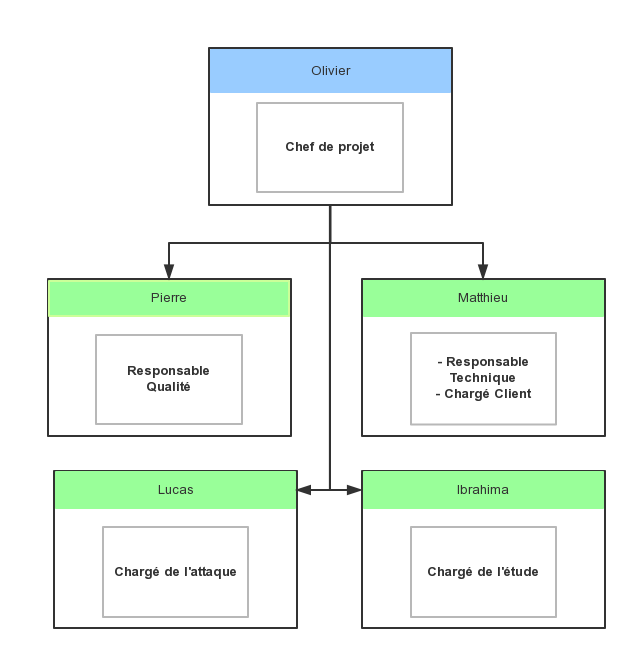
\includegraphics[scale=0.30]{guipgteam.png}
  \end{center}
\end{frame}
\subsection{Projet}
\begin{frame}
    \frametitle{\color{white}Projet}
    \begin{block}{Interface graphique : GuiPG}
      \begin{itemize}
        \item Gestion d'un trousseau de clé gpg.
        \item Actions cryptographiques.
        \item Représentation de la toile de confiance.
        \item Visualisation des commandes nécessaire pour chaque actions.
      \end{itemize}

    \end{block}
    \begin{block}{Étude de GnuPG}
    \begin{itemize}
      \item Documentation sur les possibilités de GnuPG.
      \item Guide d'utilisation de GnuPG.
    \end{itemize}
      
    \end{block}
    \begin{block}{Attaque sur les identifiants de clé}
      \begin{itemize}
        \item Forger une 2\up{nd} pré-image d'un clé sur les 4 dernier octets de son identifiant.
        \item Documentation sur les limites de GnuPG.
      \end{itemize}
    \end{block}
\end{frame}
